\documentclass[12pt,fleqn,answers]{exam}
%\usepackage{pifont}
%\usepackage{dingbat,bbding}

\usepackage{amssymb}
\usepackage[intlimits]{amsmath}
\usepackage{epsfig}
\usepackage{upgreek}
\usepackage[super]{nth}
\usepackage[colorlinks=true,linkcolor=black,anchorcolor=black,citecolor=black,filecolor=black,menucolor=black,runcolor=black,urlcolor=black]{hyperref}
\usepackage[letterpaper, margin=0.75in]{geometry}
\addpoints
\boxedpoints
\pointsinmargin
\pointname{pts}
\usepackage{tikz}
\usepackage{tkz-euclide}
\usetikzlibrary{shapes.geometric}
\usetikzlibrary{calc}
\usepackage[final]{microtype}
\frenchspacing
\usepackage[american]{babel}
\usepackage[T1]{fontenc}
\usepackage[]{fourier}
\usepackage{isomath}
\usepackage{upgreek,amsmath}
\usepackage{amssymb}
\usepackage{graphicx}

\newcommand{\dotprod}{\, {\scriptzcriptztyle\stackrel{\bullet}{{}}}\,}

\newcommand{\reals}{\mathbf{R}}
\newcommand{\lub}{\mathrm{lub}} 
\newcommand{\glb}{\mathrm{glb}} 
\newcommand{\complex}{\mathbf{C}}
\newcommand{\dom}{\mbox{dom}}
\newcommand{\range}{\mbox{range}}
\newcommand{\cover}{{\mathcal C}}
\newcommand{\integers}{\mathbf{Z}}
\newcommand{\vi}{\, \mathbf{i}}
\newcommand{\vj}{\, \mathbf{j}}
\newcommand{\vk}{\, \mathbf{k}}
\newcommand{\bi}{\, \mathbf{i}}
\newcommand{\bj}{\, \mathbf{j}}
\newcommand{\bk}{\, \mathbf{k}}
\DeclareMathOperator{\Arg}{\mathrm{Arg}}
\DeclareMathOperator{\Ln}{\mathrm{Ln}}
\newcommand{\imag}{\, \mathrm{i}}

\usepackage{graphicx}
\usepackage{color}
%\shadedsolutions
%\definecolor{SolutionColor}{rgb}{1,0.72,0.46} %{0.8,0.9,1}
\newcommand\AM{\textsc{am}}
\newcommand\PM{\textsc{pm}}
     
\newcommand{\quiz}{8}
\newcommand{\term}{Fall}
\newcommand{\due}{Thursday 21 September 13:20}
\newcommand{\class}{MATH 202, Fall \the\year}
\begin{document}
\large
\vspace{0.1in}
\noindent\makebox[3.0truein][l]{\textbf{\class}}
\textbf{Name:} \hrulefill \\
\noindent \makebox[3.0truein][l]{\textbf{In class work  \quiz}}
\textbf{Row and Seat}:\hrulefill\\
\vspace{0.1in}

\vspace{0.1in}
\noindent  In class work  \textbf{\quiz\/}  has questions \textbf{1} through  \textbf{\numquestions} \/ with a total of \textbf{\numpoints\/}  points.   
Turn in your work at the end of class  \emph{on paper}. This assignment is due \emph{\due}.

\vspace{0.1in}

\noindent \textbf{Notice:} $\cos(x)^2$ means $\left(\cos(x)\right)^2$. 
It \emph{doesn't} mean $\cos(x^2)$. Our textbook writes this 
expression as $\cos^2(x)$. Both notations are OK. Also, for
arguments that are products, it's traditional to drop the parenthesis 
for the trig functions and to write $\cos x$ for $\cos(x)$, for example.
I think this is the exit ramp to perdition (that is utter ruin).



\begin{questions} 

\question [1] Find the area of the region $\{(x,y) \mid 0 \leq y \leq \sin(x)^2 \mbox{ and } 0 \leq x \leq \uppi \}$.

\begin{solution}[2.5in]
    \begin{align*} \text{Area} &= \int_0^\uppi \sin(x)^2 \, \mathrm{d} x, && \text{(area formula)} \\
                               &= \int_0^\uppi \frac{1}{2} - \frac{1}{2} \cos(2 x) \, \mathrm{d} x, && \text{(double angle)} \\
                               &= \left. \frac{1}{2} x  - \frac{1}{4} \sin(2 x) \right |_{0}^\uppi, && \text{(known antiderivatives)}\\
                               &= \frac{\uppi}{2}. && \text{(algebra)}
    \end{align*}
\end{solution}


\question [1] Use Desmos to graph $y = \cos(x)^3$ on the interval $[0,\uppi]$. Based 
on the graph, make a pretty good guess for the numerical value of 
$\int_0^\uppi \cos(x)^3 \, \mathrm{d} x$. Duplicate the graph here 
and justify your guess.

\begin{solution}%[2.5in]

    \begin{center}
     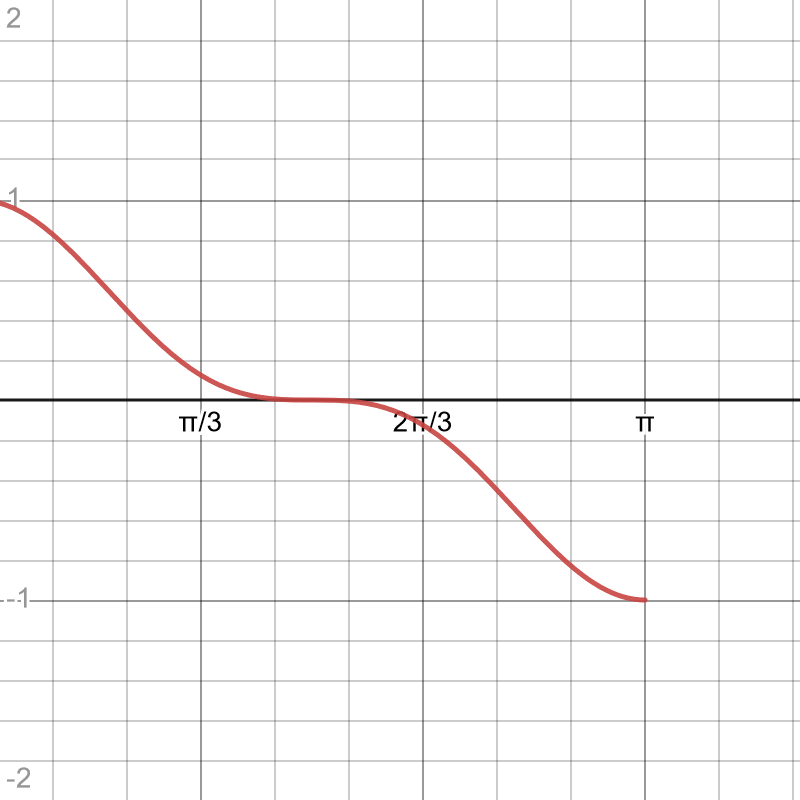
\includegraphics[scale=0.2]{desmos-graph(19).png}
    \end{center}
The area that the graph bounds that is below the x-axis appears to 
equal the area the graph bounds that is above the x-axis. My guess 
is that $\int_0^\uppi \cos(x)^3 \, \mathrm{d} x = 0$. 

\quad We could prove this by making a change of variable $x = z + \uppi/2$
and showing that the new integrand is odd and the new interval is
symmetric with respect to the origin.
\end{solution}
\newpage
\question [1] Find the numerical value of $\int_0^\uppi \cos(x)^3 \, \mathrm{d} x$.
\begin{solution}[2.5in] Let's first find an antiderivative 
    and second find the value of the definite integral.
\begin{align*}
  \int \cos(x)^3 \, \mathrm{d} x &= \int \cos(x) (1-\sin(x)^2) \, \mathrm{d} x, \\
                                 &= \int 1 - z^2 \, \mathrm{d}z &&(z = \sin(x) \text{ and } \mathrm{d}z = \cos(x) \mathrm{d} x)\\
                                 &= z - \frac{1}{3} z^3,\\
                                 &= \cos(x ) - \frac{1}{3} \cos(x)^3
  \end{align*}                    
So $\int_0^\uppi \cos(x)^3 \, \mathrm{d} x  = 0$.
\end{solution}

\newpage 
\question Use the identities
\begin{align*}
    \sin{(x)} \cos{(y)} &= \frac{\sin{\left( y+x\right) }-\sin{\left( y-x\right) }}{2}, \\
    \sin{(x)} \sin{(y)} &=  -\frac{\cos{\left( y+x\right) }-\cos{\left( y-x\right) }}{2}, \\
    \cos{(x)} \cos{(y)} &= \frac{\cos{\left( y+x\right) }+\cos{\left( y-x\right) }}{2}  
\end{align*}
to find the values of each of the following definite integrals

\begin{parts}
\part [1] $\int_0^{2 \uppi} \sin(5 x) \cos(x) \, \mathrm{d} x.$
\begin{solution}[2.5in]
\begin{equation*}
\int_0^{2 \uppi} \sin(5 x) \cos(x) \, \mathrm{d} x  = \int_0^{2 \uppi}  \frac{\sin{\left( 6 x\right) }+\sin{\left( 4 x\right) }}{2} \, \mathrm{d} x
=\left . -\frac{\cos{\left( 6 x\right) }}{12}-\frac{\cos{\left( 4 x\right) }}{8} \right |_0^{2 \uppi} = 0.
\end{equation*}
Actually for any integer $n$, we have $\int_0^{2 \uppi} \sin(n x) \, \mathrm{d} x = 0$.
Using that fact, we don't even need the antiderivative to determine 
that the value is zero.
\end{solution}

\part [1] $\int_0^{2 \uppi} \cos(5 x) \cos(x) \, \mathrm{d} x.$
\begin{solution}[2.5in]
Let's use the nice fact that for any nonzero integer $n$, we have $\int_0^{2 \uppi} \cos(n x) \, \mathrm{d} x = 0$
\begin{equation*}
\int_0^{2 \uppi} \cos(5 x) \cos(x) \, \mathrm{d} x = \int_0^{2 \uppi} \frac{\cos{\left( 6 x\right) }+\cos{\left( 4 x\right) }}{2} \, \mathrm{d} x 
= 0.
\end{equation*}
\end{solution}



\part [1] $\int_0^{2 \uppi} \cos(5 x)^2  \, \mathrm{d} x.$

\begin{solution}%[2.5in]
Again, use the nice fact that for any nonzero integer $n$, we have $\int_0^{2 \uppi} \cos(n x) \, \mathrm{d} x = 0$.
\begin{equation*}
\int_0^{2 \uppi} \cos(5 x)^2  \, \mathrm{d} x = \int_0^{2 \uppi} \frac{1}{2} + \frac{1}{2} \cos(10 x)  \, \mathrm{d} x = \uppi.
\end{equation*}
\end{solution}
\end{parts}
\end{questions}

\end{document}

